\section{Molecular Cavity and Surface Construction\label{sec:MolcSurface}}
This chapter describes the implementation of the molecular surface and cavity construction as
proposed by B. Delley\cite{Delley2006}.

\subsection{Molecular Surface Model}
Delley used for the molecular surface the zero-isosurface of a ball-and-stick-like
model function $F(\pmb{r})$ that varies continuously with the position $\pmb{r}_i$
and radii $R_i$ of the atoms. $F(\pmb{r})$ is given by
\begin{align}
  F(\pmb{r}) = 1+\sum_i f\left(\frac{(\pmb{r}-\pmb{r}_i)^2-R_i^2}{2R_sR_i} \right)
                +\sum_{i\neq j} f\left( \frac{\left[\pmb{r}-\pmb{r}_z(ij)\right]^2-R_z^2(ij)}{2R_s \max(R_z, 1.0~\text{au})} \right),
  \label{eq:delleyModelFunction}
\end{align}
where the auxiliary function $f(x)$ is given by
\begin{align}
  f(x) = -\exp(-\alpha x) + ax + b x^2.
\end{align}
The parameters $a$ and $b$ are obtained from the boundary conditions
$f(4/\alpha) = 0$ and $f^\prime(4/\alpha) = 0$. The radius of the solvent
probe is given by $R_s$. The parameter $R_z(ij)$ is the radius of a cylinder
that touches the spheres $i$ and $j$ as well as the solvent probe with radius
$R_s$, which in turn touches both spheres $i$ and $j$. It is given
with $S_i = R_i + R_s$ and $d_{ij} = |\pmb{r}_i-\pmb{r}_j|$ by
\begin{align}
  R_z(ij) = \sqrt{S_i^2 - \left( \frac{S_i^2+d_{ij}^2-S_j^2}{2d_{ij}} \right)^2}-R_s.
\end{align}
The parameter $\pmb{r}_z(ij)$ is the point of the orthogonal projection of the
point $\pmb{r}$ onto the bond between the spheres $i$ and $j$. If this projection
does not lie between spheres $i$ and $j$, $\pmb{r}_z(ij)$ is defined as the respective
bond end $\pmb{r}_i$ or $\pmb{r}_j$.
The bond part of the model (third term in Eq.~[\ref{eq:delleyModelFunction})] is restricted
to pairs $ij$ for which $d_{ij} \leq S_i+S_j$.


The model function $F(\pmb{r})$ can be understood as placing a function
$1-\exp\left[-\alpha (r-R)\right]$ on every atom and on every bond of the molecule.
Thus, $F(\pmb{r})$ will have large negative values within the molecule, a value of
$0$ at the molecular surface and a value of $1$ far outside the molecule. The parameter
$\alpha$ controls how sharp the superposition of functions from different spheres or
cylinders is. It is typically set to $\alpha = 50.0$. For small values of $\alpha$ the
surface may become blurred.

\subsection{Molecular Surface Discretization}
For the application of continuum solvation models\cite{Tomasi2005} it is necessary to
discretize the surface into small areas with one representative point each, so-called tesserae.
This is achieved by atom-wise projection of spherical integration grids to the molecular
surface as shown in Fig.~\ref{fig:delleySurfaceConstruction}(a). The normal vectors $\pmb{n}_p$
at the position of the grid point $\pmb{r}_p$, which are needed for some continuum models, are obtained as
normalized vectors with the direction of $\left.\nabla F(\pmb{r})\right|_{\pmb{r}=\pmb{r}_p}$.
In \textsc{Serenity} the standard spherical grid point distributions by Lebedev and Laikov are used.
\begin{figure}
	\centering
	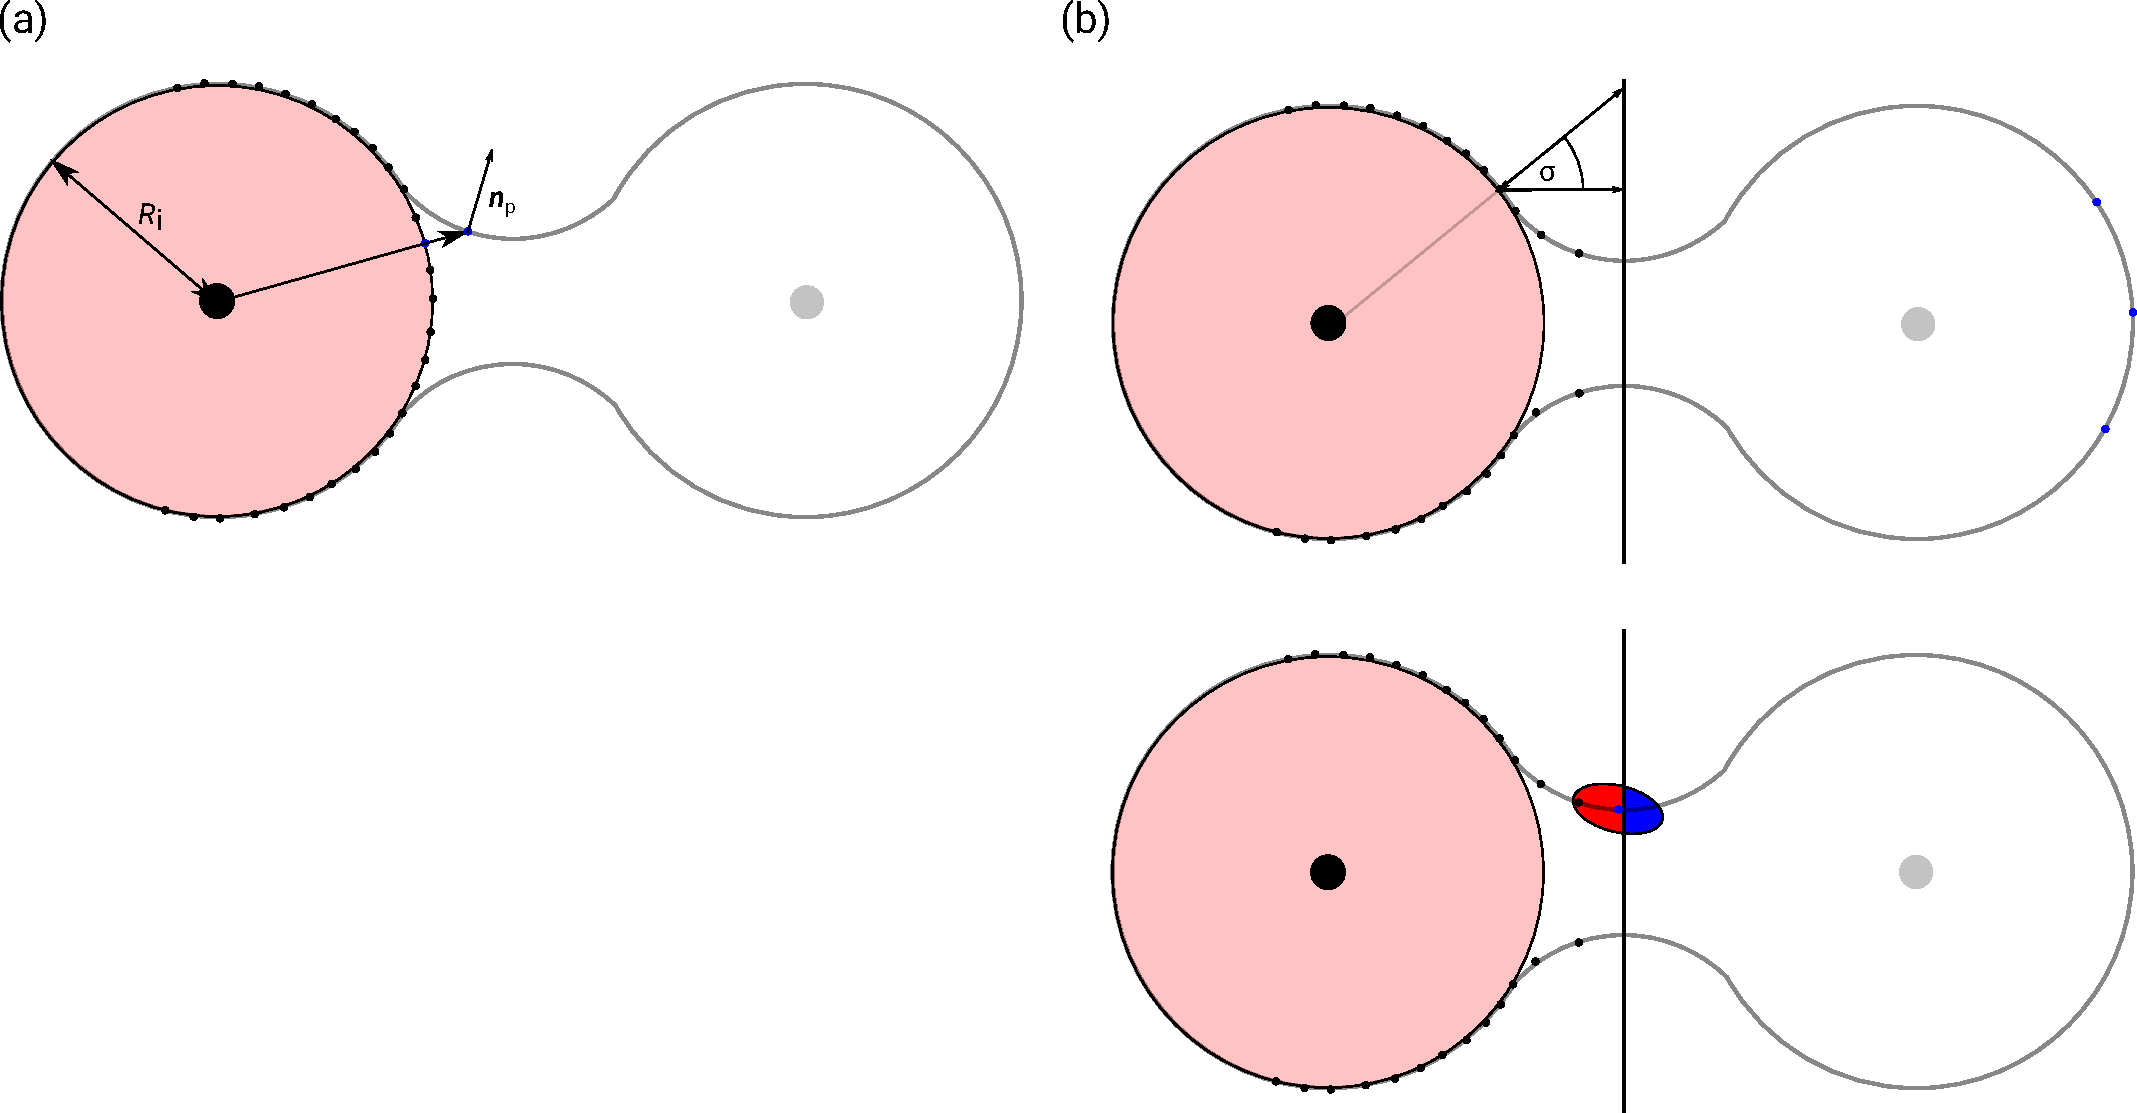
\includegraphics[width=0.95\textwidth]{figs/delleyFigure.pdf}
	\caption{Schematic of the surface mesh construction for a diatomic molecule.
			 (a) Projection of the spherical grid points to the molecular surface, and
			     construction of the normal vector $\pmb{n}_p$.
			 (b) Area scaling and cutting for grid points on the bond part of the molecular
			     surface.}
	\label{fig:delleySurfaceConstruction}
\end{figure}

The initial weights or areas $A_p^\prime$ associated to each point are calculated as
\begin{align}
	A_p^\prime = 4.0\pi A_{i,p}^{u}|\pmb{r}_p-\pmb{r}_i|^2,
\end{align}
where $A_{i,p}^{u}$ is the weight of the grid point on the unit sphere surrounding sphere $i$.
These weights are then scaled by the skew projection on the bond plane as $A_p^s = \sin(\sigma) A_p^\prime$
(see Fig.~\ref{fig:delleySurfaceConstruction}(b)) if they fall on the bond part of the surface
($\pmb{r}_z(ij) \neq \pmb{r}_i$ and $\pmb{r}_z(ij) \neq \pmb{r}_j$) and a bond between the spheres exists.
We then define planes $P(ij)$ orthogonal to each bond $ij$ (plane normal vectors
$\pmb{n}_\mathrm{bond} = \frac{\pmb{r}_i-\pmb{r}_j}{|\pmb{r}_i-\pmb{r}_j|}$) which contain the points
$\pmb{c}_\mathrm{bond} = \frac{R_i}{R_i+R_j} \pmb{r}_i +\frac{R_j}{R_i+R_j} \pmb{r}_j$, which
are the weighted centers of the bonds. We then consider each point on a bond to be an ellipse with
radial vectors $\pmb{r}_1$ and $\pmb{r}_2$ ($\pmb{r}_1^\dagger\pmb{r}_2 = 0$) given as
\begin{align}
	\pmb{r} = \pmb{r}_1 \cos(t) + \pmb{r}_2 \sin(t),~t\in [0,2\pi].
\end{align}

The ellipse construction is illustrated in Fig.~\ref{fig:ellipseConstruction}.
The direction of $\pmb{r}_1$ is obtained as the direction $\pmb{d}_s$ of the intersection between
the plane on the original sphere (its normal vector is equal to the vector $\pmb{n}_\mathrm{pro}$
used for the projection of the point to the surface) and the plane containing
the projected point, described by the normal vector $\pmb{n}_p$. The direction of $\pmb{r}_2$ is obtained by
requiring that $\pmb{r}_2$ is orthogonal to $\pmb{r}_1$ and $\pmb{n}_p$.

The length of the radial vectors is calculated by projecting a point on the circle
on the initial sphere to the plane on the molecular surface as shown in Fig.~\ref{fig:ellipseConstruction}
for $\pmb{r}_1$. The same procedure is applied for $\pmb{r}_2$. The vectors are then scaled such that
the ellipse contains the area $A_p^s$.


\begin{figure}[!ht]
	\centering
	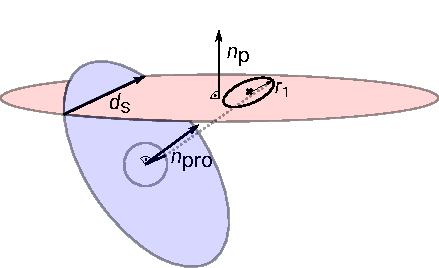
\includegraphics[width=0.8\textwidth]{figs/ellipseConstruction.pdf}
	\caption{Illustration of the ellipse construction for the area scaling.
	         The direction of the intersection between the plane on the initial sphere ($blue$)
	         and the plane on the molecular surface $red$ is denoted with $\pmb{d}_s$.
	         The vector $\pmb{r}_1$ is obtained by going from the center of the circle on the
	         initial sphere in direction of $\pmb{d}_s$ according to the area of the circle.
	         Then a line is constructed containing this point with direction $\pmb{n}_\mathrm{pro}$,
	         and the intersection with the $red$ plane is calculated. The same is done for $\pmb{r}_2$.
	         Both vectors are then scaled such that the ellipse has the desired area.}
	\label{fig:ellipseConstruction}
\end{figure}

If an ellipse is cut by a plane $P(ij)$ [see Fig.~\ref{fig:delleySurfaceConstruction}(b)], the area and the center
of gravity $\pmb{r}_{p,\mathrm{grav}}$ not hidden by the plane from the perspective of the owning atom is calculated.
If the ellipse is completely hidden by the plane, the point is dropped.
The center of gravity is projected back to the molecular surface along the direction
$\pmb{r}_{p,\mathrm{grav}}-\pmb{r}_i$ and a new ellipse is constructed. This procedure is repeated for all $j$ bonding
with $i$. This construction ensures that all points remain on the bond side of their initial atoms.
